\chapter{Interpreting co-expressive verbal extensions} \label{ch:interpretation}

Chapter \ref{ch:functions} provides a detailed description of the meanings that are found to be co-expressed with directional meaning in verbal extensions in Chadic languages. These include meanings in the categories of associated motion\index{associated motion}, location, tense-aspect and benefactive, as well as idiomatic combinations of extensions and verb roots. In a purely compositional approach to morphosyntax, it might be assumed that it would be possible to predict what non-directional meaning would appear in different contexts, perhaps depending on the lexical subclass of the predicate or the type of event described. While there are clear trends as to how directional extensions are used across Chadic languages, the interpretation of directional extensions seems to be a highly context-sensitive affair which is often idiosyncratic and seemingly unpredictable. 

As a simplified starting point, it is sometimes assumed that when a morpheme that can have a directional function occurs with a motion verb, it will express direction. For example, in a study of directionals in six African languages,  \citet[62]{belkadiAssociatedMotionDeictic2015} notes that ``most of the languages surveyed seem to have a clear-cut dichotomy whereby motion verbs trigger directional uses, while other classes of verbs trigger [associated motion] uses.'' However, Belkadi notes some exceptions, including (\ref{ex:taqb}) from Taqbaylit (Berber). In Taqbaylit, the clitic \textit{d} typically has a directional function with motion verbs, and can have a subsequent associated motion\index{associated motion} interpretation in other contexts. However, in (\ref{ex:taqb}), the verb \textit{ʕum} `swim' combined with \textit{d} does not allow a directional interpretation in spite of the verb denoting an event typically thought of as a type of motion event \citep[see also][]{belkadiDeicticDirectionalitySpace2015}. 

\ea\label{ex:taqb}
\langinfo{Taqbaylit verb \textit{ʕum} `swim' with ventive marker}{}{\cite[53]{belkadiAssociatedMotionDeictic2015}} \\
\gll i-ʕum =d \\
\gl{3}\gl{sg}.\gl{m}-swim.\gl{prf} =\gl{vent} \\
\glt `He (went somewhere) swam and came back (to the location of the speaker or to his house).' \newline
\textbf{not:} `He swam (towards or to the location of the speaker).'
\z

Another complication is that there are verb-directional combinations that allow more than one interpretation. This is even the case in English where the combination \textit{throw up} could either be used directionally to describe the path of motion of a thrown object or be used idiomatically to refer to vomiting. Compare the example in (\ref{ex:huba2}) where the outward extension combined with the verb \textit{vàk} `throw' can either be translated with a directional meaning (the path of the thrown object is outward) or with an aspectual (totality) meaning. 

\ea\label{ex:huba2}
\langinfo{\hyperref[huba]{Huba} verb \textit{vàk} `throw' with outward suffix}{}{\cite[113]{muazuGrammarKilbaLanguage2009}} \\
\gll vàk-bìyà	 \\
throw-\gl{out} \\
\glt `You throw out/all.'
\z 

This chapter looks at the translations of directional extensions across Chadic languages to examine which verb glosses are more likely to be found with a directional interpretation of the verbal extension, and which non-directional co-expressed meanings appear with which verb roots. Since the data for this study is taken from a variety of sources, a significant caveat is that the verbs are categorized according to whatever gloss each linguist gave them, and in some cases, these had to be translated into English from French or German. Since there are no objective criteria for establishing how to gloss verbs across Chadic languages, these classifications by gloss are only approximations of verbal semantics. Some glosses were slightly modified for clarity, and three standardized glosses have been introduced. The gloss `\textsc{motion}' replaces the source gloss where it is clear that the verb is a general motion verb without entailing any directional meaning (=`go/come'). The gloss `enter/exit' is used where it is clear that the verb is a general boundary-crossing motion verb which expresses crossing a bounded space without entailing whether the direction is inward or outward. The gloss `buy/sell' is used where a verb can have either meaning (without verbal morphology marking the distinction, see Chapter \ref{ch:buysell}).  

A second caveat is that there is not an equal amount of data from each language in the sample. Each source presents a different set of combinations of verbs and directionals, and these do not overlap enough for there to be a subset of verb-extension combinations that are found across most sources. For this reason, the results presented here are not representative in any statistically significant sense. This descriptive overview of the available data serves two purposes. First, it presents a general picture of how directional extensions are interpreted across a wide range of verbs. Second, this overview lays out some of the issues that arise in the description of Chadic languages, particularly drawing attention to how a systematic study of the semantic variation that occurs when verbs interact with directional extensions can be an insightful approach to understanding the lexical semantics of verbs. 

Table \ref{tab:interpretation1} and Table \ref{tab:interpretation2} show the 65 glosses that appear most frequently on a verb with a directional extension in the data. The first column in each row shows the gloss, and the number in the column ``Total'' is the total number of unique triples of verb root, directional extension, and interpretation of the directional extension for that gloss across all languages in the data. In cases where a single language has more than one verb root with the same gloss, each verb root is counted separately. If the same verb root occurs with more than one kind of directional extension, these are also counted as separate types. For example, if a verb glossed `put' in a particular language is attested with a ventive extension and with an itive extension, that is counted as two examples of a verb glossed `put' combining with a directional extension. If the same verb-extension pair allows more than one interpretation of the directional extension, as in (\ref{ex:huba2}), these are also counted as separate types. 

The column labeled DIR shows how many unique verrb-extension pairs are found with a directional interpretation. If a verb root appears in multiple examples from a particular language with the same directional extension and the same interpretation, these are only counted once per language. In order to display the data more succinctly, the other columns in each table cluster together related interpretations of verb-extension combinations. The column labeled ``AM/LOC'' includes all verb-extension combinations with a translation that is locative, associated motion\index{associated motion} or resultative (caused) motion. The column CAM counts pairs that have a caused accompanied motion interpretation (Chapter \ref{ch:CAM}). The column ``Non-motion'' combines all non-motion interpretations including aspectual interpretations, idiomatic uses and a few cases of fictive motion. The final category, the one in which the majority of unique combinations of a verb and a directional extension are found, are cases where it is unclear what the function of the directional extension is. The data from Table \ref{tab:interpretation1} and Table \ref{tab:interpretation2} are visualized in a horizontal bar graph in Figure \ref{fig:interpretation}.

%data in tab:interpretation1 from python file Interpretation
\begin{table}
	\caption{Interpretations of directional extensions by verb gloss (1/2)}
	\label{tab:interpretation1}
	\begin{tabular}{lrrrrrr} % add l for every additional column or remove as necessary
		\lsptoprule
	gloss &   	DIR &  AM/LOC &   CAM &  Non-motion &  Unclear &  Total \\
\midrule
put         &   49 &             0 &    0 &           3 &       12 &     64 \\
come        &   43 &             0 &    2 &           1 &        6 &     52 \\
go          &   42 &             0 &    1 &           2 &        5 &     50 \\
return      &   38 &             0 &    0 &           0 &        7 &     45 \\
throw       &   35 &             0 &    0 &           1 &        3 &     39 \\
pour        &   27 &             0 &    0 &           2 &        5 &     34 \\
\textsc{motion}      &   27 &             0 &    0 &           0 &        5 &     32 \\
run         &   21 &             0 &    0 &           1 &        2 &     24 \\
carry       &   19 &             0 &    0 &           0 &        2 &     21 \\
fall        &   17 &             1 &    0 &           1 &       11 &     30 \\
send        &   17 &             0 &    0 &           0 &        3 &     20 \\
arrive      &   15 &             0 &    0 &           0 &        0 &     15 \\
push        &   15 &             0 &    0 &           1 &        2 &     18 \\
leave       &   14 &             0 &    0 &           1 &        3 &     18 \\
exit        &   13 &             0 &    0 &           0 &        1 &     14 \\
jump        &   13 &             0 &    0 &           0 &        3 &     16 \\
enter       &   12 &             0 &    0 &           0 &        2 &     14 \\
pull        &   12 &             0 &    0 &           0 &        2 &     14 \\
climb       &    9 &             0 &    0 &           0 &        3 &     12 \\
give        &    8 &             0 &    0 &           1 &        8 &     17 \\
descend     &    8 &             0 &    0 &           0 &        3 &     11 \\
go-\textsc{caus}     &    7 &             0 &    0 &           0 &        0 &      7 \\
enter/exit  &    7 &             0 &    0 &           0 &        0 &      7 \\
move(tr.)   &    6 &             0 &    0 &           0 &        1 &      7 \\
sweep       &    5 &             0 &    0 &           0 &        4 &      9 \\
gather      &    3 &             0 &    2 &           0 &       14 &     19 \\
shoot       &    2 &             2 &    0 &           0 &        4 &      8 \\
close       &    2 &             2 &    0 &           1 &        3 &      8 \\
hit         &    2 &             1 &    0 &           5 &        4 &     12 \\
remove      &    2 &             1 &    1 &           0 &        5 &      9 \\
open        &    2 &             0 &    0 &           0 &        8 &     10 \\
search      &    1 &             5 &    0 &           0 &        7 &     13 \\
draw(water) &    1 &             4 &    0 &           0 &        7 &     12 \\
		\lspbottomrule
	\end{tabular}
\end{table}

\begin{table}
	\caption{Interpretations of directional extensions by verb gloss (2/2)}
	\label{tab:interpretation2}
	\begin{tabular}{lrrrrrr} % add l for every additional column or remove as necessary
		\lsptoprule
		gloss &   DIR &  AM/LOC &   CAM &  Non-motion &  Unclear &  Total \\
		\midrule
sow         &    1 &             2 &    0 &           2 &        3 &      8 \\
call        &    0 &            15 &    0 &           0 &        7 &     22 \\
buy         &    0 &            11 &    0 &           7 &       10 &     28 \\
bind        &    0 &             9 &    0 &           0 &        3 &     12 \\
eat         &    0 &             9 &    0 &           2 &       11 &     22 \\
catch       &    0 &             9 &    2 &           2 &       12 &     25 \\
cut         &    0 &             8 &    0 &           3 &       19 &     30 \\
steal       &    0 &             7 &    0 &           1 &        7 &     15 \\
tie         &    0 &             7 &    1 &           5 &        5 &     18 \\
cook        &    0 &             6 &    0 &           2 &        7 &     15 \\
buy/sell    &    0 &             5 &    0 &           6 &        2 &     13 \\
wash        &    0 &             4 &    0 &           1 &        5 &     10 \\
break       &    0 &             3 &    0 &           7 &       22 &     32 \\
burn        &    0 &             3 &    0 &           1 &        4 &      8 \\
kill        &    0 &             3 &    0 &           0 &        5 &      8 \\
drink       &    0 &             3 &    0 &           2 &        5 &     10 \\
do          &    0 &             3 &    1 &           5 &       17 &     26 \\
plant       &    0 &             2 &    0 &           0 &        5 &      7 \\
find        &    0 &             2 &    1 &           1 &        8 &     12 \\
finish      &    0 &             1 &    0 &           2 &        8 &     11 \\
make        &    0 &             1 &    0 &           0 &        6 &      7 \\
see         &    0 &             1 &    0 &           1 &       10 &     12 \\
leave(tr.)   &    0 &             1 &    0 &           0 &        8 &      9 \\
know        &    0 &             1 &    0 &           1 &        6 &      8 \\
untie       &    0 &             1 &    0 &           1 &        5 &      7 \\
die         &    0 &             0 &    0 &           0 &        7 &      7 \\
tell        &    0 &             0 &    0 &           0 &        7 &      7 \\
give.birth  &    0 &             0 &    0 &           0 &        7 &      7 \\
build       &    0 &             0 &    0 &           0 &        8 &      8 \\
seek        &    0 &             0 &    0 &           1 &        6 &      7 \\
take        &    0 &             0 &   59 &           4 &       16 &     79 \\
		\lspbottomrule
	\end{tabular}
\end{table}

\begin{figure}
	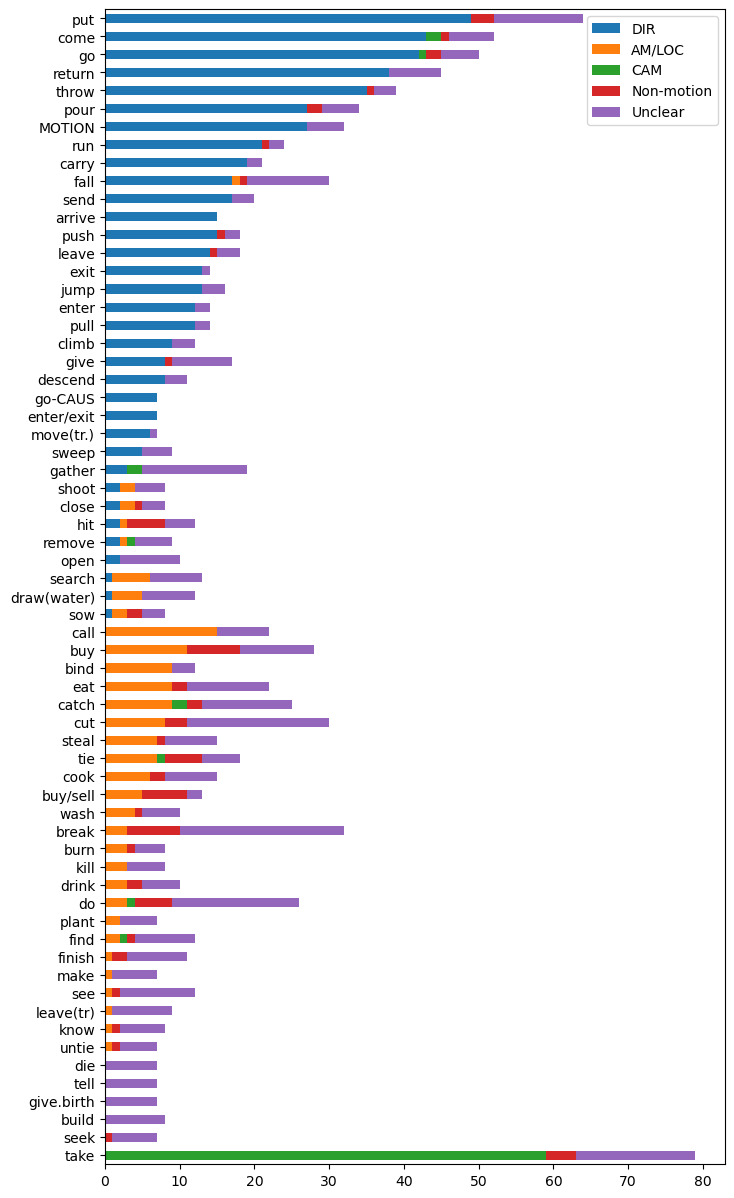
\includegraphics[width=0.85\textwidth]{figures/interpretation.png}
	\caption{Interpretations of extensions by verb gloss}
	\label{fig:interpretation}
\end{figure}

There are three general trends in how directional extensions tend to be interpreted when combined with a particular class of verb roots. First, directional extensions combined with prototypical motion verbs, unsurprisingly, nearly always result in a directional interpretation. However, there are a number of exceptions to this in the data. These are discussed in Section \ref{sec:interpretingmotion}. There is another group of verbs which are not typical motion verbs, but which can be given a directional reading in which some aspect of the event is construed as occurring along a literal path of motion. These verbs are discussed in Section \ref{sec:orientation}. They do not necessarily always have a directional interpretation, and are also commonly found with a subsequent motion interpretation. Finally, there are several verbs which are often presented as typical cases where a directional extension is given a subsequent motion interpretation. However, as discussed in Section \ref{sec:interpretingAM}, the same verb roots combined with directional extensions are also frequently found with non-motion interpretations. It cannot be assumed that the combination of a directional extensions with such verbs will always result in a subsequent motion interpretation.

\section{Motion verbs} \label{sec:interpretingmotion}

At the top of Table \ref{tab:interpretation1} and the top of Figure \ref{fig:interpretation} it can be seen that directional extensions most frequently have a directional interpretation when combined with prototypical verbs of motion such as `go', `return', `run' ,`jump', `exit' and `throw'. The high frequency of examples with a verb glossed `put' is possibly due to Chadic languages having several verbs for specific types of putting events which are all translated by English `put'. Directional extensions show a very strong bias toward a directional function when combined with motion verbs, but there are a number of exceptions. The exceptions are mostly idiomatic verb-extension combinations, as shown in (\ref{ex:mada0}), (\ref{ex:psik0}) and (\ref{ex:gude0}).  

\ea\label{ex:mada0}
\langinfo{\hyperref[mada]{Mada} verb \textit{pā} `put' with `side' suffix}{}{\cite[62]{ernstkurdiTenseAspectMood2016}} \\
\gll Ná-pā-fā-ŋ-và ma ...	\\
1\gl{sg}-put-\gl{side}-\gl{appl}-\gl{refl}.\gl{ipfv} \gl{top}	\\
\glt `I start...'

\ex\label{ex:psik0}
\langinfo{\hyperref[psik]{Psikye} verb \textit{dze} `go' with upward suffix}{}{\cite[117]{smithKapsikiLanguage1969}} \\
\gll nya malé dze-mé va cɛ	\\
\gl{dem} woman go-\gl{up} near house \\
\glt `This woman is standing near her house.'

\ex\label{ex:gude0}
\langinfo{\hyperref[gude]{Gude} verb \textit{hwa} `run' with ventive suffix}{}{\cite[203]{hoskinsonGrammarDictionaryGude1983}} \\
\gll hwa-ya	\\ 
run-\gl{vent}	\\ 
\glt `grow horizontally (of vine)'
\z 

Only in one case, shown in (\ref{ex:huba2}) above, is there a clear aspectual interpretation of a combination of a motion verb and directional extension. There is also only one example of a motion verb combining with a directional extension with an associated motion\index{associated motion} interpretation, rather than a directional interpretation. In (\ref{ex:pero4}), the \hyperref[pero]{Pero} verb \textit{cúg} `fall' combines with a ventive extension and is translated with a subsequent motion interpretation.\footnote{In the \hyperref[haus]{Hausa} data, there is also an example in which the verb \textit{sāw-ō} `put-\textsc{vent}' is translated as `put here, put on and come' \citep[662]{newmanHausaLanguageEncyclopedic2000}. The first translation is taken as a directional meaning when the verb has a transitive (caused) motion meaning. The second translation is taken as a separate meaning of the verb root which could be paraphrased as `dress'. In this case, the predicate is describing a non-motion event, and so the subsequent motion interpretation of the directional is as expected.} 

\ea\label{ex:pero4}
\langinfo{\hyperref[pero]{Pero} verb \textit{cúg} `fall' with ventive suffix}{}{\cite[94]{frajzyngierGrammarPero1989}} \\
\gll  cúg-ínà	tù	púccù \\
fall-\gl{compl}.\gl{vent}	\gl{prep} there	 \\
\glt `He fell there and subsequently came here.'
\z 

Finally, in \hyperref[glav]{Glavda}, the motion verbs \textit{s} `come' and \textit{d} `go' can combine with directional extensions to express caused accompanied motion. However, it should be noted that this meaning only arises with the transitive directional extensions which are distinguished from other extensions by beginning with \textit{d} (Chapter \ref{ch:identifying2}, Section \ref{sec:allomorphy}). Compare (\ref{ex:glav01}), where the verb \textit{s} `come' combines with the regular downward suffix and has a directional interpretation, with (\ref{ex:glav02}), where the same verb is combined with the transitive downward suffix and has a caused accompanied motion interpretation (`bring'), as further discussed in Chapter \ref{ch:CAM}. 

\ea\label{ex:glav01}
\langinfo{\hyperref[glav]{Glavda} verb \textit{s-} `come' with downward suffix}{}{\cite[]{owensGlavdaRuralUrban2011}} \\
\gll sə-xi	\\
come-\gl{down} \\
\glt `come down'

\ex\label{ex:glav02}
\langinfo{\hyperref[glav]{Glavda} verb \textit{s-} `come' with transitive downward suffix}{}{\cite[]{owensGlavdaRuralUrban2011}} \\
\gll sə-dií	\\
come-\gl{down}.\gl{tr}		\\
\glt `bring down'
\z 

\section{Orientation of an event} \label{sec:orientation}

There are a number of verb roots that are not typical motion verbs, but which can have a directional interpretation where the event they describe is construed as occurring along a path of motion. These include `shoot', `close', `remove', `hit', `open', `search', `draw (water)' and `sow'. Alternatively, these verbs can combine with a directional extension which is interpreted as a subsequent motion following the main event. 

For example, in (\ref{ex:haus02}), a \hyperref[haus]{Hausa} verb root glossed `shoot' is combined with a ventive marker and the interpretation is that the event takes place along a ventive path of motion, specifically that the projectile moves along a path of motion toward the speaker. Note that the existence of this projectile is entailed by the meaning of the verb, but it is not necessarily an argument of the verb. In (\ref{ex:bole0}), a \hyperref[bole]{Bole} verb root glossed `shoot' is combined with a ventive marker, but here the interpretation is subsequent ventive motion (or no translocative motion at all), rather than a directional interpretation.

\ea\label{ex:haus02}
\langinfo{\hyperref[haus]{Hausa} verb \textit{har̃b} `shoot' with ventive extension}{}{\cite[662]{newmanHausaLanguageEncyclopedic2000}} \\
\gll bā sā̀ har̃b-ô-wā	\\
?? ?? shoot-\gl{vent}-\gl{nmlz} \\
\glt `They are not shooting (at it) in this direction.'

\ex\label{ex:bole0}
\langinfo{\hyperref[bole]{Bole} verb \textit{màt} `shoot' with ventive extension}{}{\cite[39]{schuhBoleTangaleLanguagesBauchi1978}} \\
\gll mù màt-ín-kò	\\
1\gl{pl} shoot-\gl{vent}-\gl{pfv} \\
\glt `We shot (and brought).' or simply `We shot.'		
\z 

As another example, compare (\ref{ex:ngiz0}) and (\ref{ex:gude03}). In (\ref{ex:ngiz0}), a \hyperref[ngiz]{Ngizim} verb root glossed `close' is combined with a ventive extension with a directional interpretation. The path of motion that the door moves along is toward the deictic center. In (\ref{ex:gude03}), a \hyperref[gude]{Gude} verb root glossed `close' is combined with a ventive extension and the interpretation is subsequent ventive motion, rather than directional. 

\ea\label{ex:ngiz0}
\langinfo{\hyperref[ngiz]{Ngizim} verb \textit{cim} `close' with ventive extension}{}{\cite[81]{schuhAspectsNgizimSyntax1972}} \\
\gll miya mavgi da-cim-ayi	\\
mouth door \textsc{stative}-close-\gl{vent}		\\
\glt `The door is closed (this way).'

\ex\label{ex:gude03}
\langinfo{\hyperref[gude]{Gude} verb \textit{pya'} `close' with ventive extension}{}{\cite[98]{hoskinsonGrammarDictionaryGude1983}} \\
\gll  pya'-a	\\
close-\gl{vent}	\\
\glt `close and come'	
\z 

In data from \hyperref[bana]{Bana}, the verb root \textit{pla} `search' combined with a ventive extension can have either a directional or a subsequent motion interpretation. In (\ref{ex:bana0}), the interpretation is directional, while in (\ref{ex:bana01}), the interpretation is subsequent motion. 

\ea\label{ex:bana0}
\langinfo{\hyperref[bana]{Bana} verb \textit{pla} `search' with ventive extension}{}{\cite[44]{zuchGrammaireExercicesLangue1977}} \\
\gll  pla-ke vlé	\\
seek-\gl{vent} rabbit	\\
\glt `Go after the rabbit (in our direction)!' \newline
[French: `\textit{Chasse le lapin} (\textit{dans notre direction}) !']

\ex\label{ex:bana01}
\langinfo{\hyperref[bana]{Bana} verb \textit{pla} `search' with ventive extension}{}{\cite[44]{zuchGrammaireExercicesLangue1977}} \\
\gll pla-ke zer̂we!	\\
seek-\gl{vent} child	\\
\glt `Go look for the child (and bring him toward me)!' \newline 
[French: `\textit{Va chercher l'enfant} (\textit{et amène-le vers moi}) !']
\z 

The Bara examples in (\ref{ex:bana0}) and (\ref{ex:bana01}) are particularly interesting because both examples are of the same verb root from the same language, yet with two different interpretations of the directional extension. \citet[184]{belkadiDeicticDirectionalityAssociated2021} observes that ``motion and directional or path interpretations appear to be in complementary distributions across single languages.'' In other words, in most cases the available evidence allows an assumption that speakers of a particular language tend to be consistent in whether they allow a directional interpretation or an associated motion interpretation of a particular verb root -- even if there is variation across languages in regard to which verb roots fall into which category. As the Bara examples are the only counterexample in the dataset, \citet[184]{belkadiDeicticDirectionalityAssociated2021} appears to be correct that it is ``extremely rare for a form to be ambiguous between a directional interpretation and an additional motion event interpretation with a single verb [in a single language].'' However, it it also very possible that with more research on this topic, more counterexamples will be discovered.

\section{Subsequent motion and non-motion interpretations} \label{sec:interpretingAM}

Among those cases where a directional extension combines with a non-motion verb, one attested result is for the directional extension to receive a motion interpretation (other than directional) such as subsequent motion (Chapter \ref{ch:functions}, Section \ref{sec:comotion}). This interpretation is extremely common with verb roots that have glosses like `call', `buy', `bind', `eat', `catch', `cut' and `steal'. However, it is not the case that directional extensions always have a subsequent motion interpretation when combined with a non-motion verb. There are several non-motion verb roots that occur (cross-linguistically) with a directional extension that is given a non-motion interpretation. In other words, there is not a simple dichotomy between direction and associated motion in the interpretation of directional extensions across Chadic languages. 

A common case of non-motion interpretations of directional extensions is the idiomatic interpretation of specific verb-extension combinations. The most commonly found idiomatic use of directional extensions is the case of verbs glossed `buy' or `buy/sell'. In these cases, directional extensions take on the function of distinguishing between buying and selling events (Chapter \ref{ch:buysell}). In languages where this has not occurred, directional extensions tend to have a subsequent motion interpretation with a `buy' verb. 

Aspectual functions can also create a situation in which non-motion interpretations appear rather than subsequent motion interpretations. For example, in (\ref{ex:dghw01}) from \hyperref[dghw]{Dghwede}, the outward extension combined with the verb `cook' has a subsequent motion interpretation. In contrast, in \hyperref[bura]{Bura} the outward extension allows a aspectual interpretation, as shown in (\ref{ex:bura04}) where it combines with a verb glossed `cook'. 

\ea\label{ex:dghw01}
\langinfo{\hyperref[dghw]{Dghwede} verb \textit{tə́gə̀} `cook' with ventive outward extension}{}{\cite[6]{frickVerbalSystemDghwede1978}} \\
\gll kâ' tə́gə̀-díle kfì	\\
\gl{narr} cook-\gl{vent}.\gl{out} food		\\
\glt `She cooked food and brought it out.'

\ex\label{ex:bura04}
\langinfo{\hyperref[bura]{Bura} verb \textit{bwa} `cook' with outward extension}{}{\cite[4]{blenchBuraVerbalExtensions2010}} \\
\gll bwa-ɓəla	\\
cook-\gl{out}	\\
\glt `to cook thoroughly'
\z 

In \hyperref[bole]{Bole}, the ventive extension has a number of possible interpretations. In addition to a directional function, it can have a subsequent motion interpretation, a locative interpretation, a beneficiary interpretation or an idiomatic interpretation. In (\ref{ex:bole01}), the ventive form of the verb `eat' has a subsequent motion interpretation. In contrast, in (\ref{ex:bole02}), the ventive form of the verb `eat' has a beneficiary interpretation. Note that in (\ref{ex:bole02}) the verb also has a pronominal suffix referencing the beneficiary. This is part of the context that suggests (or perhaps even requires) a benefactive interpretation of the ventive extension. 

\ea\label{ex:bole01}
\langinfo{\hyperref[bole]{Bole} verb \textit{tíish} `eat' with ventive extension}{}{\cite[146]{gimbaBoleVerbMorphology2000}} \\
\gll à tíish-àakí-d-dí	\\
?? eat-\gl{vent}-\gl{vent}-\gl{add}	\\
\glt `He eats with it and comes.'

\ex\label{ex:bole02}
\langinfo{\hyperref[bole]{Bole} verb \textit{tíish} `eat' with ventive extension}{}{\cite[142]{gimbaBoleVerbMorphology2000}} \\
\gll tí-n-ní-n-tì	\\
eat-\gl{vent}-3SG.M-\gl{vent}-\gl{compl}	\\
\glt `He has eaten for him here.'
\z 

\section{Predicting interpretation through verbal semantics}

\citet{belkadiAssociatedMotionConstructions2016,belkadiDeicticDirectionalityAssociated2021} proposes an implicational hierarchy of verbs by lexical semantic types, shown in (\ref{ex:hierarchy}). Where verbal morphology can co-express either directional meaning or associated motion\index{associated motion} (DIR/AM), the hypothesis is that DIR/AM morphemes are more likely to have a directional interpretation with the verbs higher (further left) on this hierarchy and, conversely, are more likely to have an associated motion interpretation with the verbs lower on the hierarchy. 

\ea \langinfo{\textbf{Hierarchy of verbs by semantic type}}{}{\cite[191]{belkadiDeicticDirectionalityAssociated2021}} \label{ex:hierarchy} \\
Path motion > Motion translational > Causative motion > Perception >  Activities not involving translational motion > States 
\z 

The aim of the hierarchy in (\ref{ex:hierarchy}) is to go beyond a binary division between motion events and non-motion events in predicting the interpretation of morphemes that co-express directionality and associated motion\index{associated motion}. Belkadi's ``Path motion'' category includes directional motion events encoded in verbs with meanings like `descend', `enter' and `arrive'. The ``Motion translational'' category includes manner-of-motion verbs like `run', `jump' or `swim' where the event described involves a figure moving from one location to another. 

Belkadi does not provide any quantitative results of her study of 20 African languages. The hypothesis can be applied to the data in Table \ref{tab:interpretation1} and Table \ref{tab:interpretation2} but with a null result. Looking at the interpretations of DIR/AM verbal extensions in this dataset, it can be seen that all motion verbs elicit directional interpretations. Only one ``Motion translational'' verb (`fall') and one ``Causative motion'' verb (`remove') are additionally attested with an associated motion meaning. The rarity of associated motion interpretations among motion verbs in the data means that it is not possible to establish a statistically significant difference between ``Path motion'', ``Motion translation'' and ``Causative motion'' verbs. 

Non-motion verb roots in this dataset are nearly all ``Activities not involving translational motion.'' There is only one ``Perception'' verb root and one ``States'' verb root. For this reason, it is not possible to establish whether one subtype of non-motion verb root is more likely to elicit a directional or associated motion interpretation of a DIR/AM morpheme based on this data from Chadic languages. The only significant distinction in this dataset is a dichotomy between motion and non-motion verbs. 

\citet[368]{genettiDirectionAssociatedMotion2020} also tested Belkadi's hypothesis by applying a simplified version of Belkadi's hierarchy to data from 23 Tibeto-Burman languages. They provide quantitative data in regard to the first three types of motion verbs in (\ref{ex:hierarchy}). They conclude that ``although we must be tentative due to the small number of examples, overall the Tibeto-Burman data seem to confirm Belkadi’s proposed ranking'' \citep[371]{genettiDirectionAssociatedMotion2020}. However, there are a number of issues with that claim.

According to their coding of the data, DIR/AM morphemes are least likely to have an associated motion\index{associated motion} interpretation with manner-of-motion verbs. This interpretation is found in just 1 of 26 examples (4\%). DIR/AM morphemes have an associated motion interpretation when combined with directional (path-of-motion) verbs in seven of 65 examples (11\%). Causative motion verbs combined with DIR/AM morphology result in an associated motion interpretation in 11 of 53 examples (21\%).\footnote{\citet[370]{genettiDirectionAssociatedMotion2020} do not present the percentages as given here, but instead calculate what percentage of the 19 examples of associated motion interpretations with motion verbs are from each subclass, without regard to how many total examples there are of each subclass.} According to these statistics, DIR/AM morphology is least likely to have an associated motion interpretation when combined with manner-of-motion verb roots, and, therefore, manner-of-motion verbs should actually be highest on the hierarchy ahead of directional (path-of-motion) verbs. Causative motion verbs (or transitive motion verbs) most commonly result in an associated motion interpretation of DIR/AM morphemes, and are therefore the lowest of three motion types on the hierarchy, as predicted.

Furthermore, there are three issues with the coding of data in \citet{genettiDirectionAssociatedMotion2020}. First, several activity verbs are questionably classified as (translocative) motion verbs, including verbs glossed `hunt', `plough' and `search'. Second, several instances of directional meaning are classified as concurrent associated motion\index{associated motion}. In a footnote, \citet[370]{genettiDirectionAssociatedMotion2020} acknowledge that Antoine Guillaume made them aware of this issue, but they appeal to the ``exact translation'' as the basis of their classification. Having examined the relevant examples, it appears that the distinction between directional and associated motion was made on the basis of the syntactic structure of the English translation, rather than whether the event predicated by the verb is a translocative motion event \citep[as defined by][]{guillaumeAssociatedMotionSouth2016}. Third, they include examples translated as `leave behind' as associated motion, even though the examples do not necessarily make it clear that the relevant verbal morphology predicates a motion event (although it may be implied). In summary, upon closer scrutiny, \citet{genettiDirectionAssociatedMotion2020} do not have sufficient evidence to support the idea that motion verbs can be subcategorized semantically as to whether a co-expressive DIR/AM verbal morpheme is more likely to have an associated motion or directional interpretation. 



\section{Conclusion}

The data presented in this chapter on Chadic languages support the general notion that if a co-expressive verbal morpheme can express directional meaning, it will nearly always do so when modifying a motion verb. Most exceptions involve aspectual or idiomatic interpretations. Only very rarely does an associated motion interpretation appear with a motion verb. However, the data do not support Belkadi's \citeyear{belkadiAssociatedMotionConstructions2016} proposed fine-grained universal hierarchy of semantic types of verb roots in regard to interpreting co-expressive directional morphology. 

The data from Chadic languages also highlight the diversity of possible functions other than associated motion which may be co-expressed with directional meaning. The same morphemes that co-express direction and associated motion might also co-express a third function, as discussed in Section \ref{sec:interpretingAM}. There are 26 morphemes which, in addition to expressing direction, co-express associated motion as well as at least one other non-motion function, as in the \hyperref[bole]{Bole} examples in (\ref{ex:bole01}) and (\ref{ex:bole02}) above. This complexity cannot be captured in a simple dichotomy: if motion, direction; if not, associated motion. At this point, very little is known about how speakers interpret such multi-functional morphemes. There appears to be a considerable amount variation.

The other area of complexity is that there are events which involve some type of movement that is not linguistically structured as a translocative motion event (in the sense that none of the verb's arguments are a figure on a path of motion), but which can be construed as translocative motion when a directional extension is used, as discussed in Section \ref{sec:orientation}. Speakers have considerable flexibility to either construe the event as a motion event and interpret the verbal extension as directional, or to treat the verb root as non-motion and give another interpretation to the verbal extension such as subsequent motion. 

On the one hand, there is a very clear pattern in the grammar of Chadic languages allowing a great deal of certainty in predicting how directional extensions will be interpreted when used with a motion verb. On the other hand, there is a great deal of complexity in how directional extensions are interpreted when not used with a motion verb. The complexity involved in the interpretation of co-expressive verbal extensions does not lend itself to a straightforward compositional semantic analysis and requires a richer view of how speakers compose and interpret meaning. Verbal semantics alone are not always sufficient for predicting the interpretation of co-expressive directional extensions. Whether from language to language, or within a particular language, the interpretation of directional extensions depends not only on the lexical semantics of the verb, but on other factors, including grammatical context (such as other verbal morphology) and real-world context.
